% \chapter{Analysis of the System Measurement}\label{apendice1}

% In this appendix, it is demonstrated the results of the several tests performed during the experimental analysis, with the objective to have a better evaluation of the measurement system developed for the detergent supervision. 

% According to Table \ref{table:testSummary}, the tests from Section~\ref{appendice1:first} desire to verify the behavior of the measurement system when trying different numbers of readings from the ultrasonic sensor.

% Already, for the Section~\ref{appendice1:second}, it is presented the experimental results of the measurements in order to verify the system's reliability. The range of values approached in this test are varied between 10 cm to 90 cm, in which represents the values of interest for the measurement system to operate.

% Finally, the Section~\ref{appendice1:third} illustrates the result of the analysis of the temperature influence on the capacity level measured from the device.

% \clearpage
% \section{Experimental Results}\label{appendice1:first}

% \begin{figure}[h!]
%     \centering
%     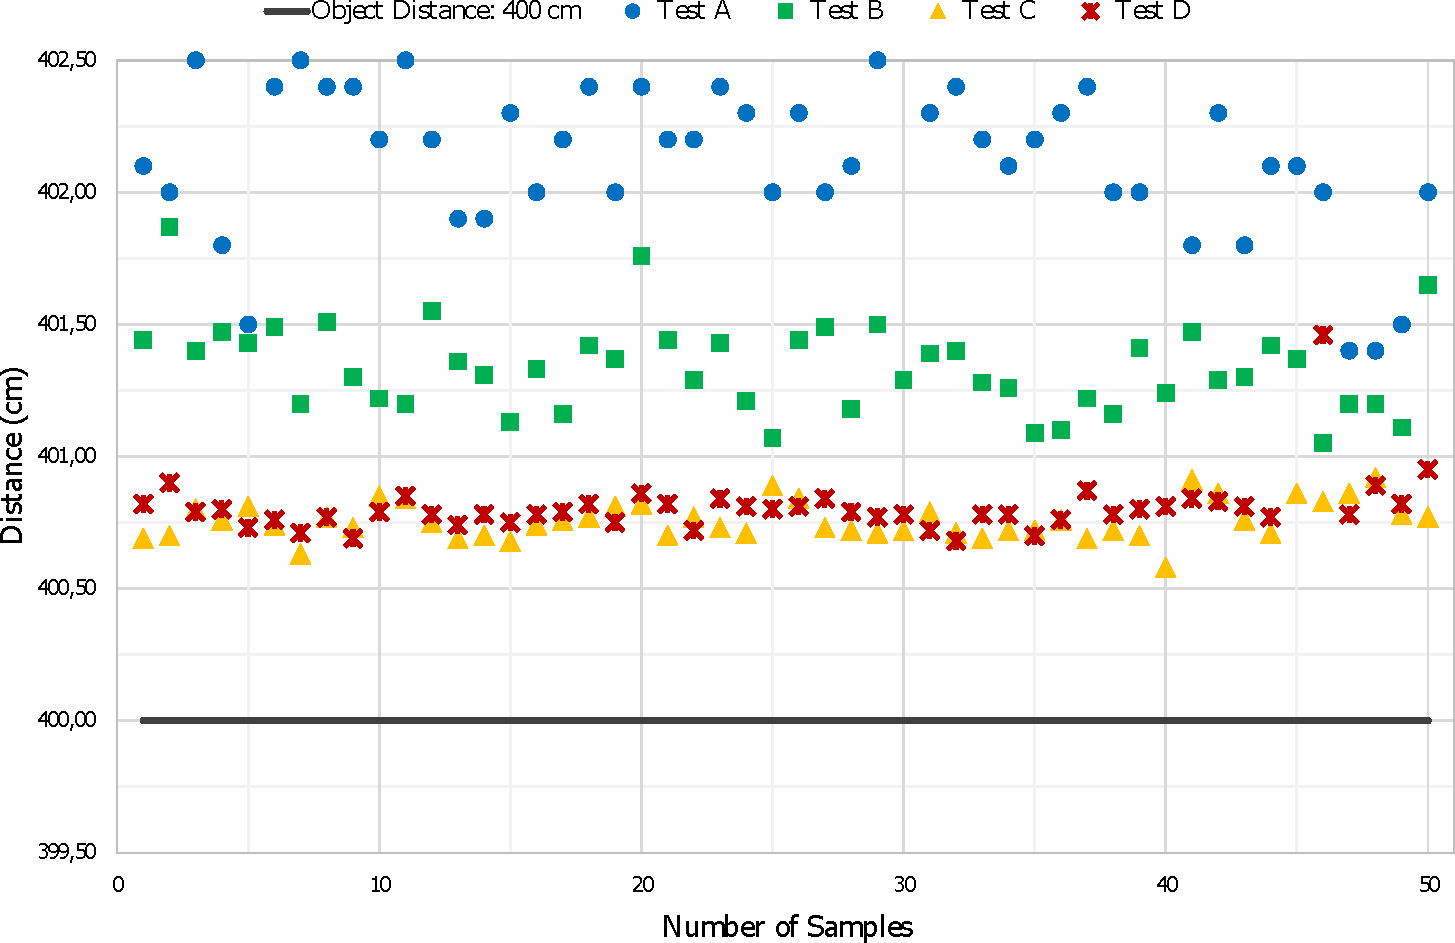
\includegraphics[scale=0.52]{images/Results/testing_methodology/400cm.pdf}
%      \caption{Analysis \#1; Object Distance: 400 cm.}
%     \label{fig:400cm}
% \end{figure}

% \begin{figure}[h!]
%     \centering
%     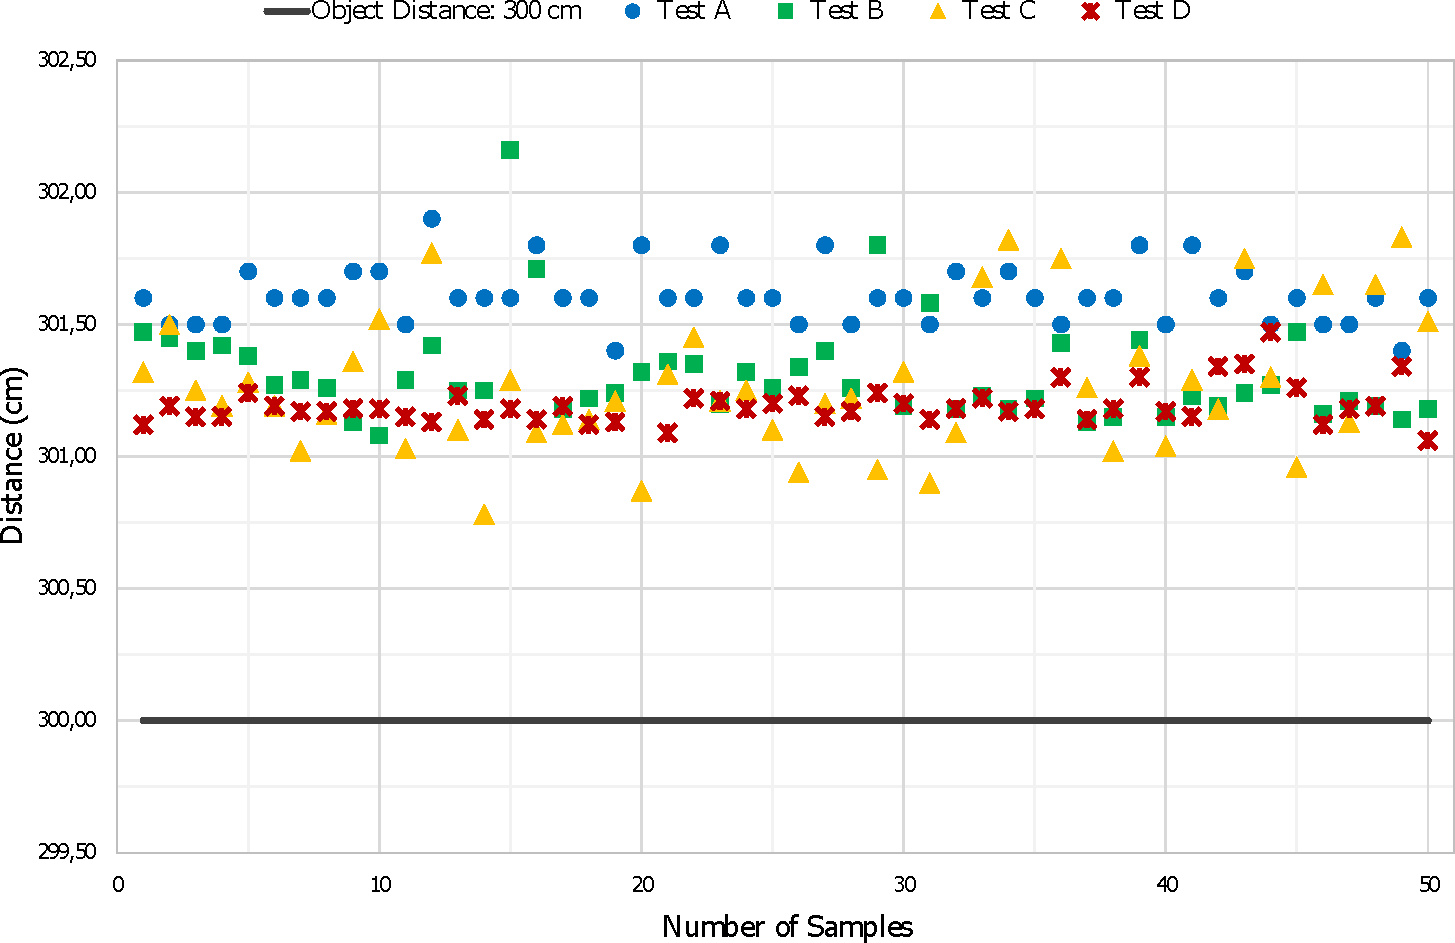
\includegraphics[scale=0.52]{images/Results/testing_methodology/300cm.pdf}
%     \caption{Analysis \#1; Object Distance: 300 cm.}
%     \label{fig:300cm}
% \end{figure}

% \begin{figure}[h!]
%     \centering
%     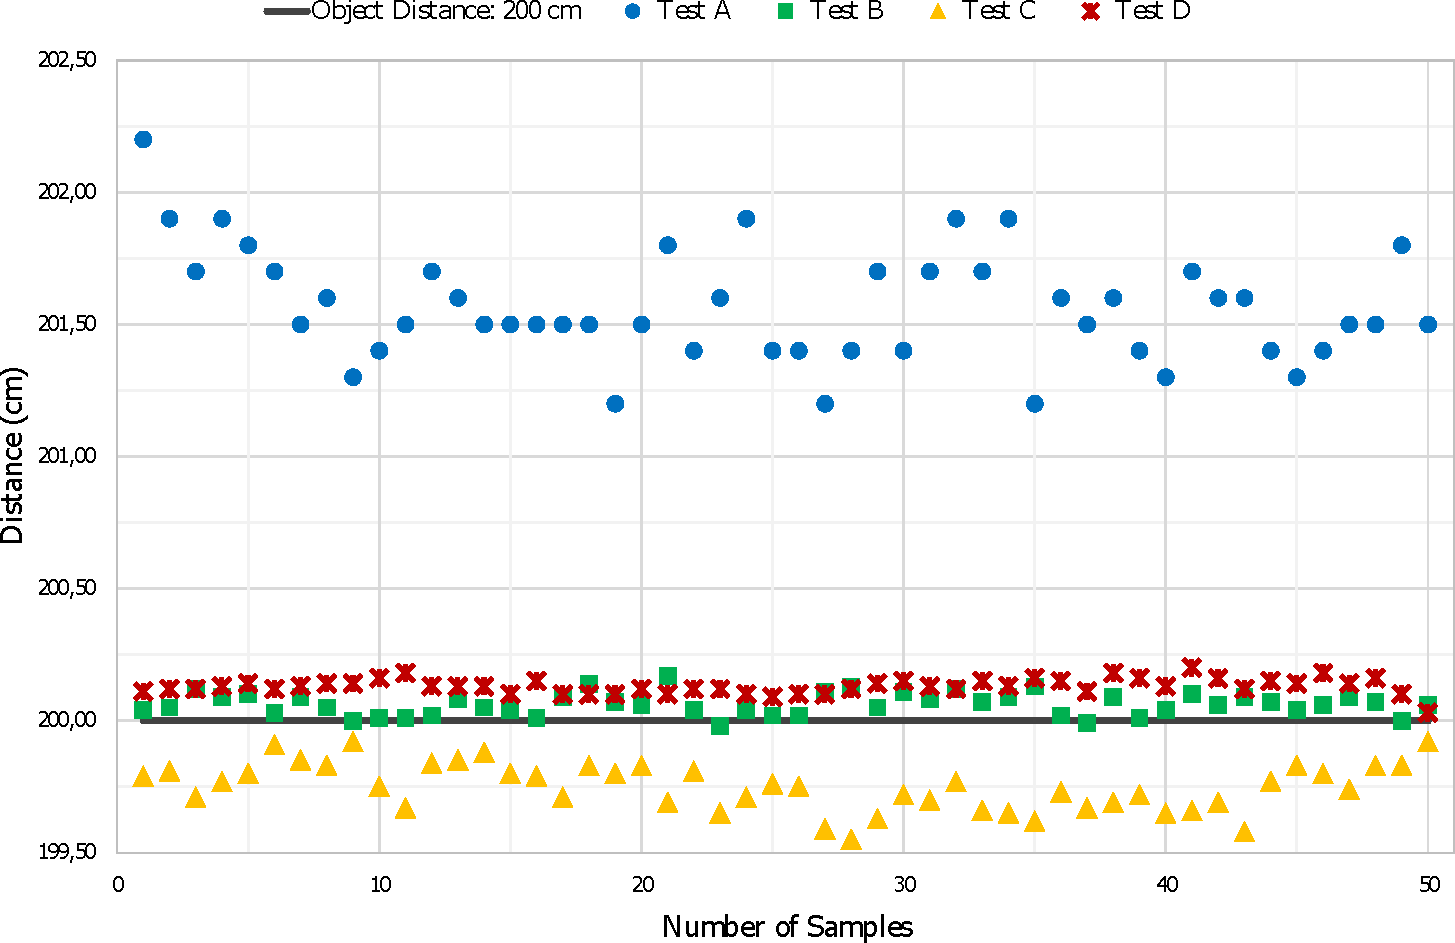
\includegraphics[scale=0.52]{images/Results/testing_methodology/200cm.pdf}
%     \caption{Analysis \#1; Object Distance: 200 cm.}
%     \label{fig:200cm}
% \end{figure}

% \begin{figure}[h!]
%     \centering
%     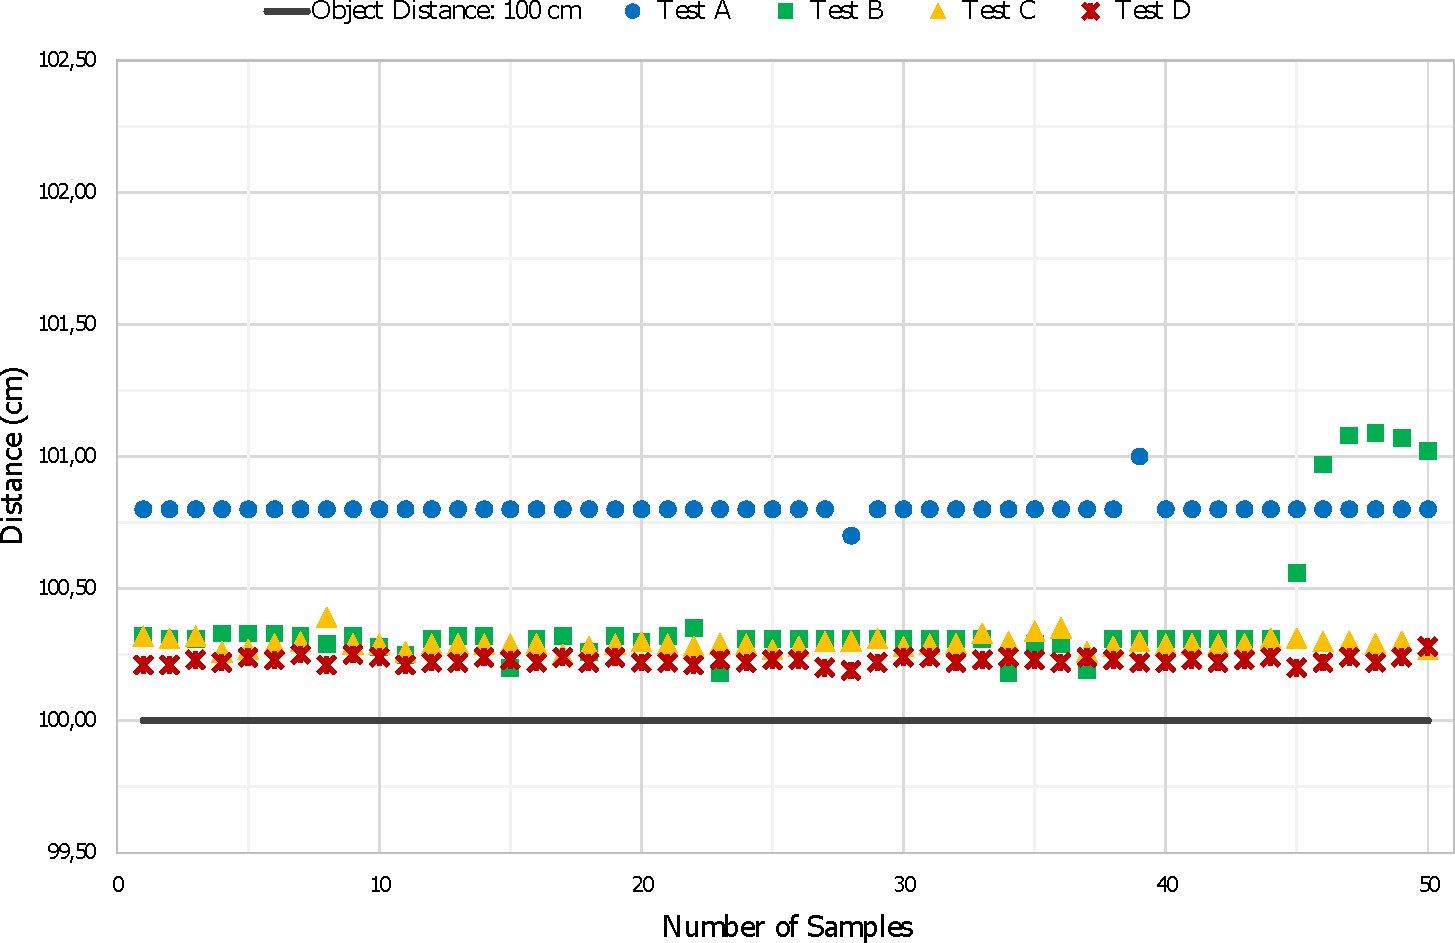
\includegraphics[scale=0.52]{images/Results/testing_methodology/100cm.pdf}
%     \caption{Analysis \#1; Object Distance: 100 cm.}
%     \label{fig:100cm}
% \end{figure}

% \begin{figure}[h!]
%     \centering
%     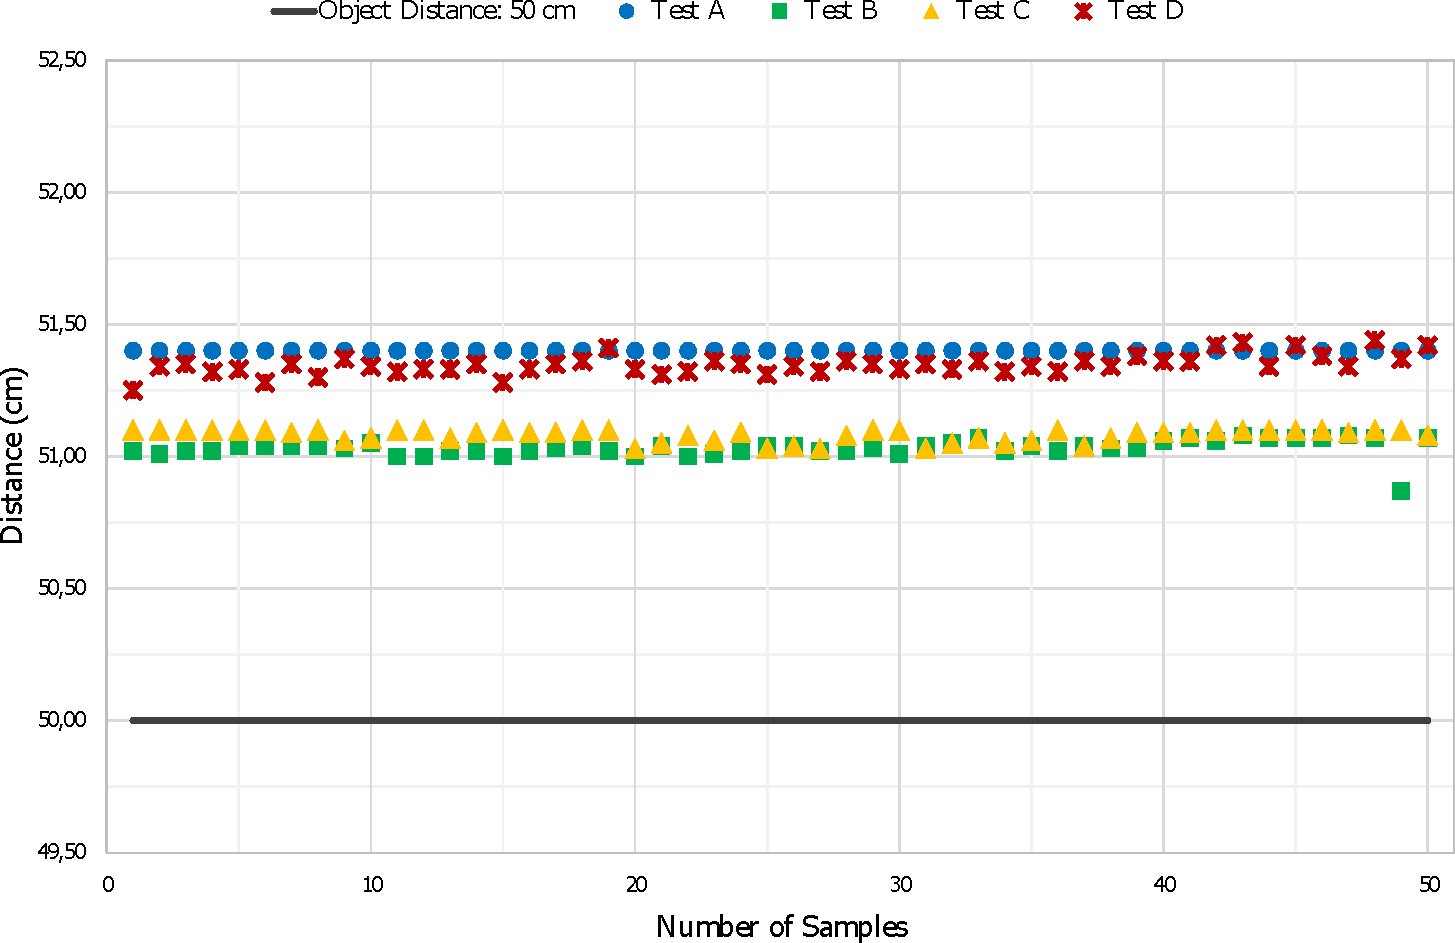
\includegraphics[scale=0.52]{images/Results/testing_methodology/50cm.pdf}
%     \caption{Analysis \#1; Object Distance: 50 cm.}
%     \label{fig:50cm}
% \end{figure}

% \begin{figure}[h!]
%     \centering
%     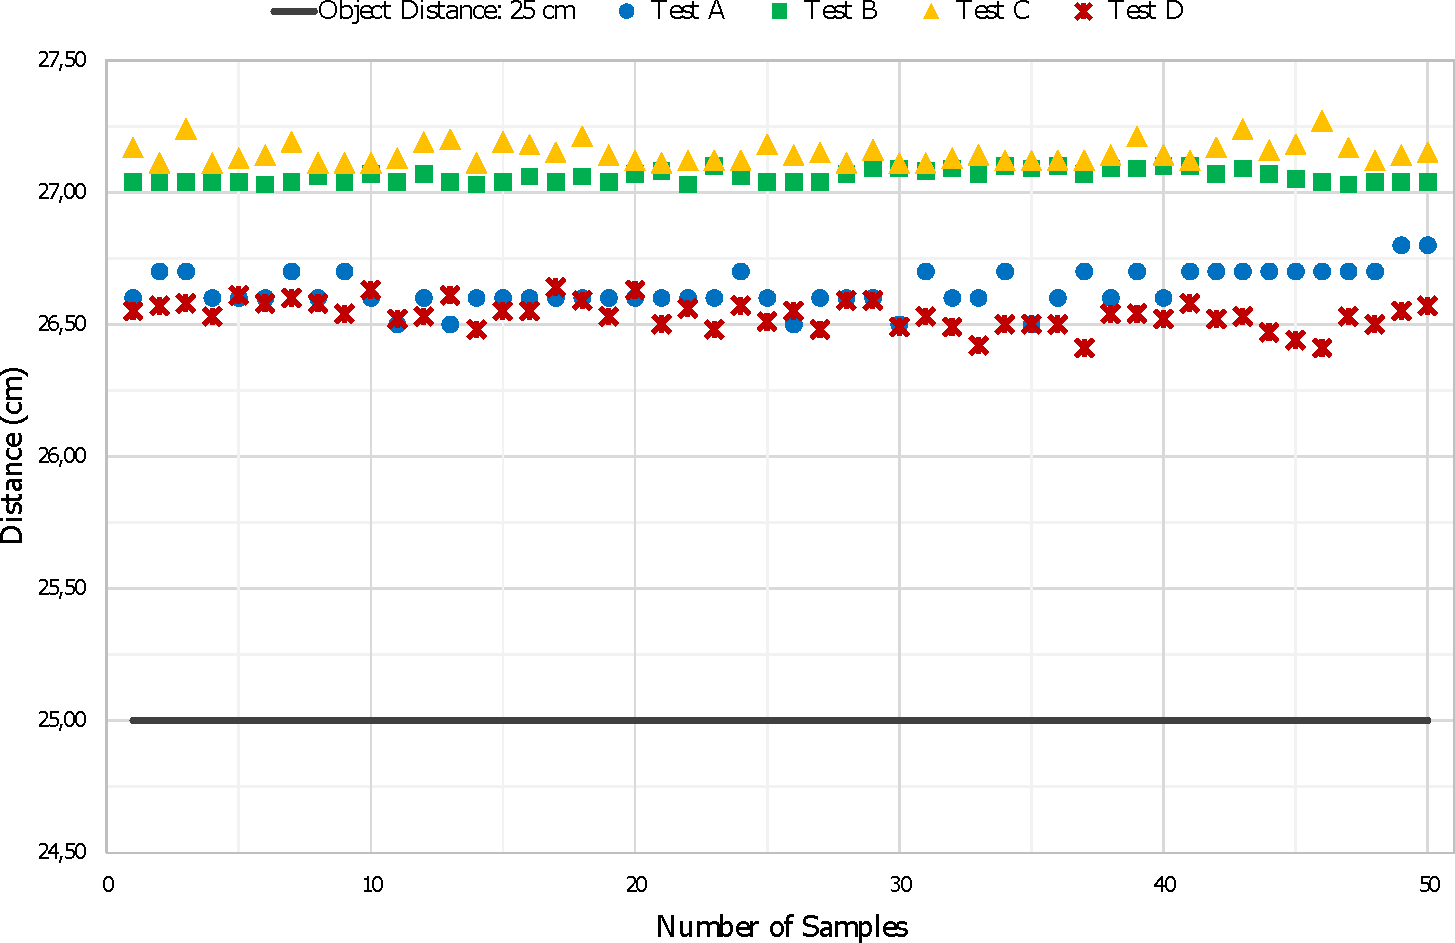
\includegraphics[scale=0.52]{images/Results/testing_methodology/25cm.pdf}
%     \caption{Analysis \#1; Object Distance: 25 cm.}
%     \label{fig:25cm}
% \end{figure}

% \begin{figure}[h!]
%     \centering
%     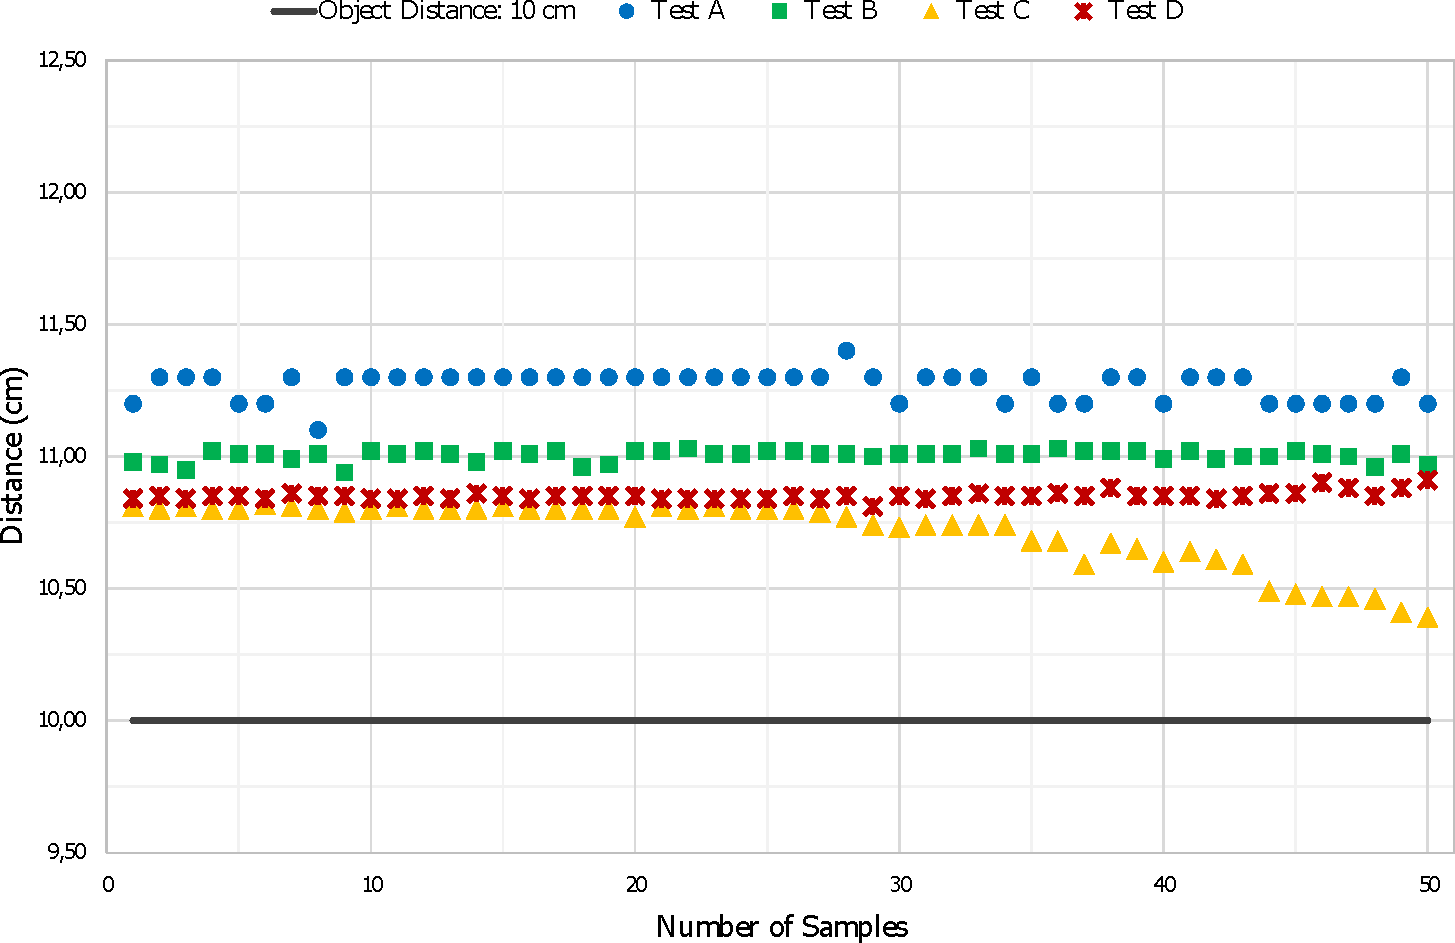
\includegraphics[scale=0.52]{images/Results/testing_methodology/10cm.pdf}
%     \caption{Analysis \#1; Object Distance: 10 cm.}
%     \label{fig:10cm}
% \end{figure}

% \begin{figure}[h!]
%     \centering
%     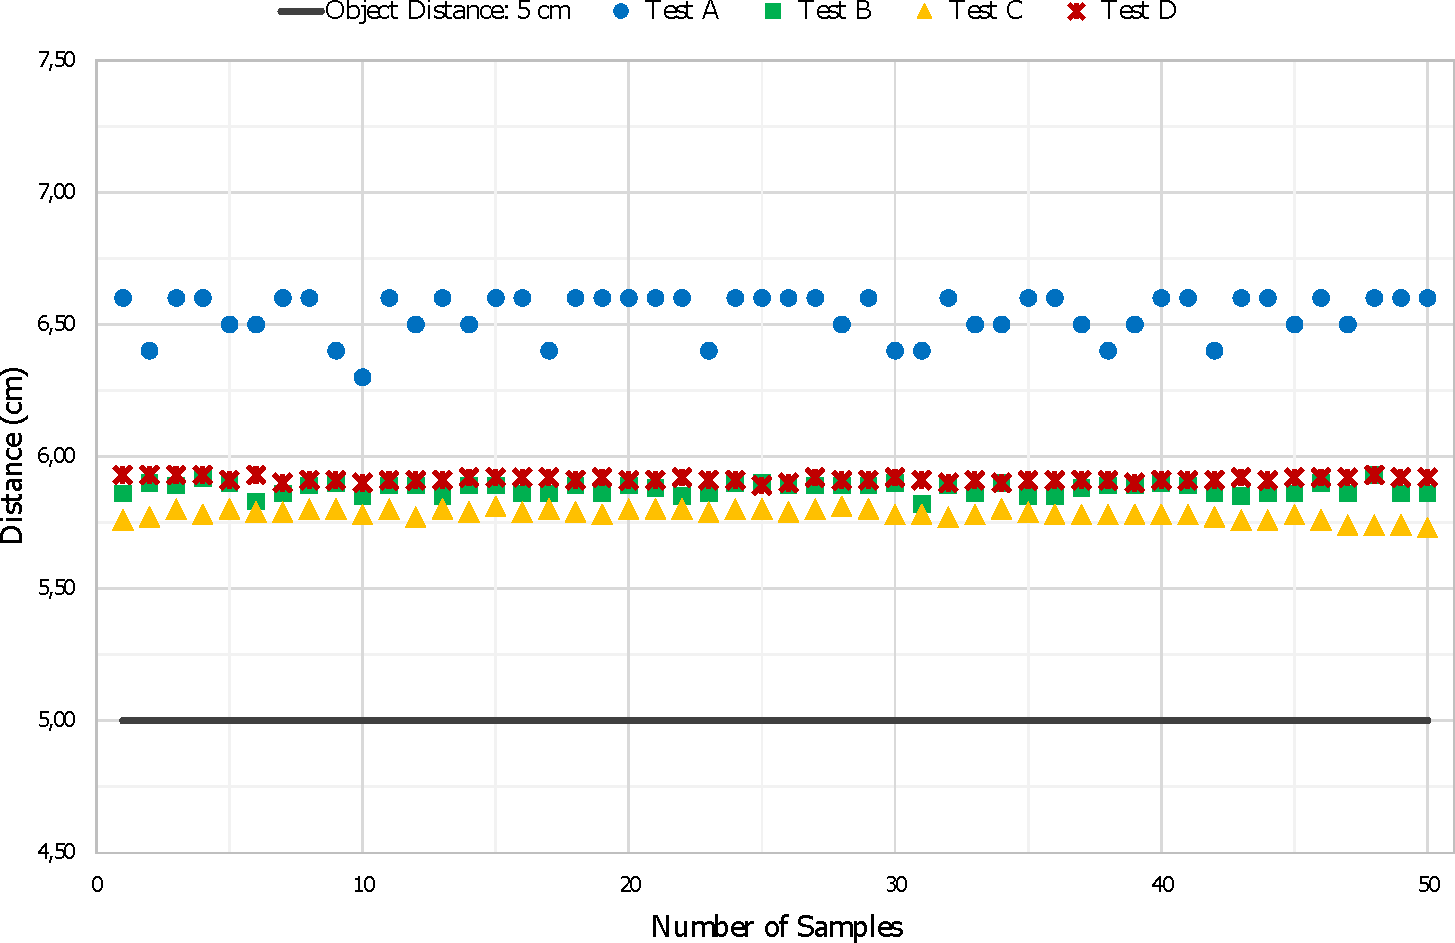
\includegraphics[scale=0.52]{images/Results/testing_methodology/5cm.pdf}
%     \caption{Analysis \#1; Object Distance: 5 cm.}
%     \label{fig:5cm}
% \end{figure}

% \clearpage
% \section{System's Reliability}\label{appendice1:second}

% \begin{figure}[h!]
%     \centering
%     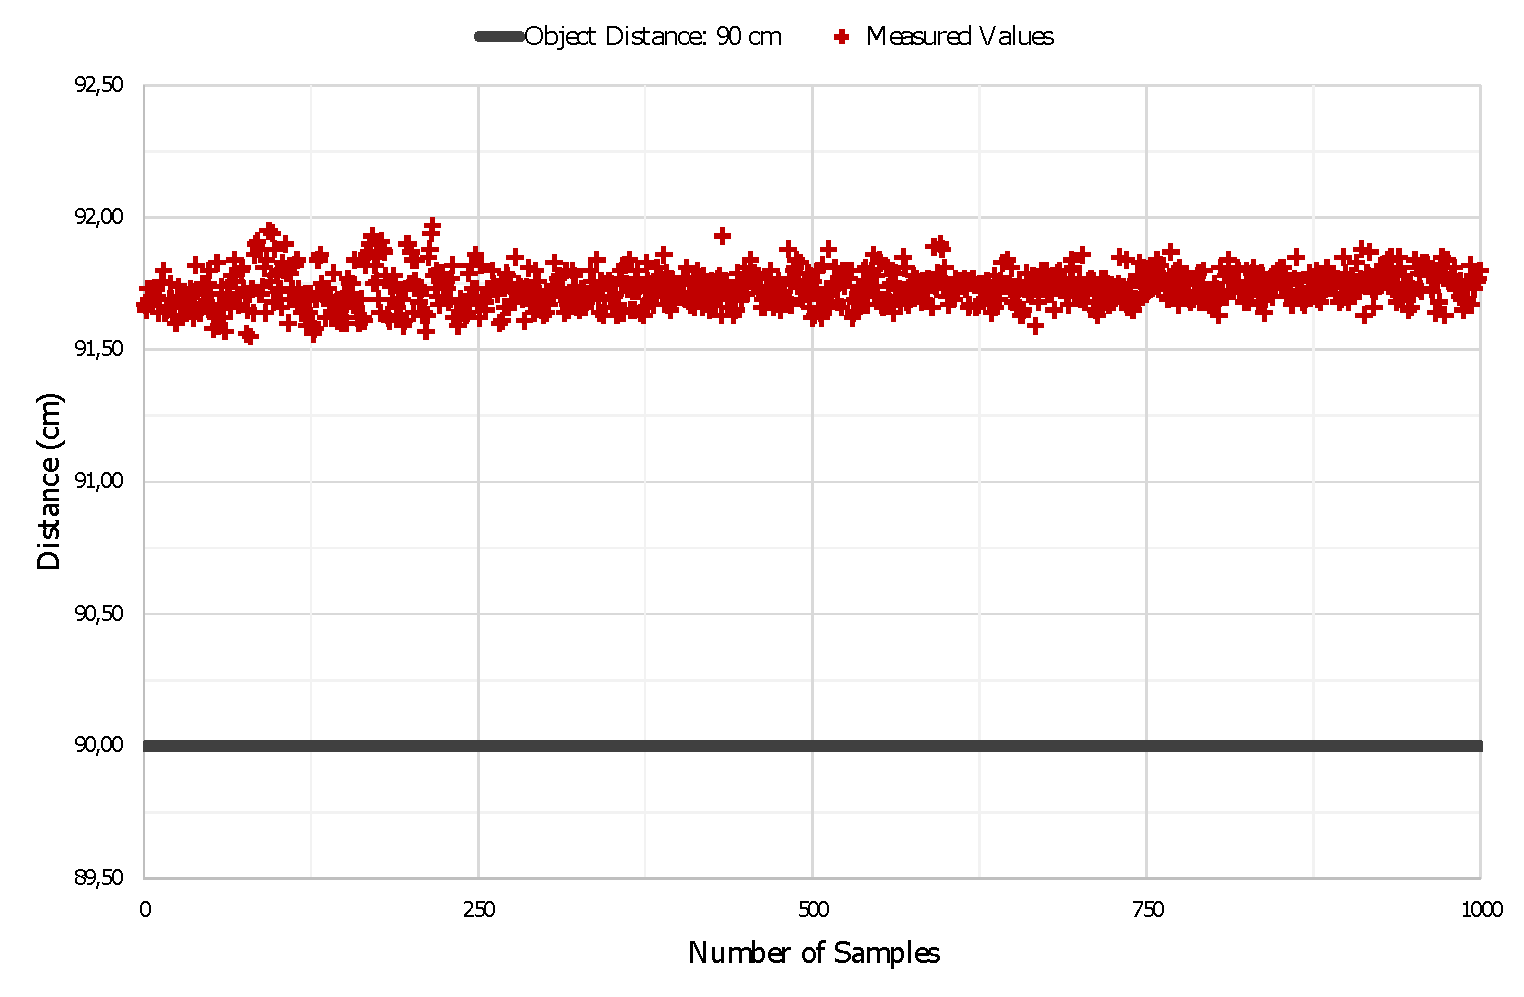
\includegraphics[scale=0.52]{images/Results/testing_methodology/conf90.pdf}
%     \caption{Analysis \#2; Object Distance: 90 cm.}
%     \label{fig:conf90}
% \end{figure}

% \begin{figure}[h!]
%     \centering
%     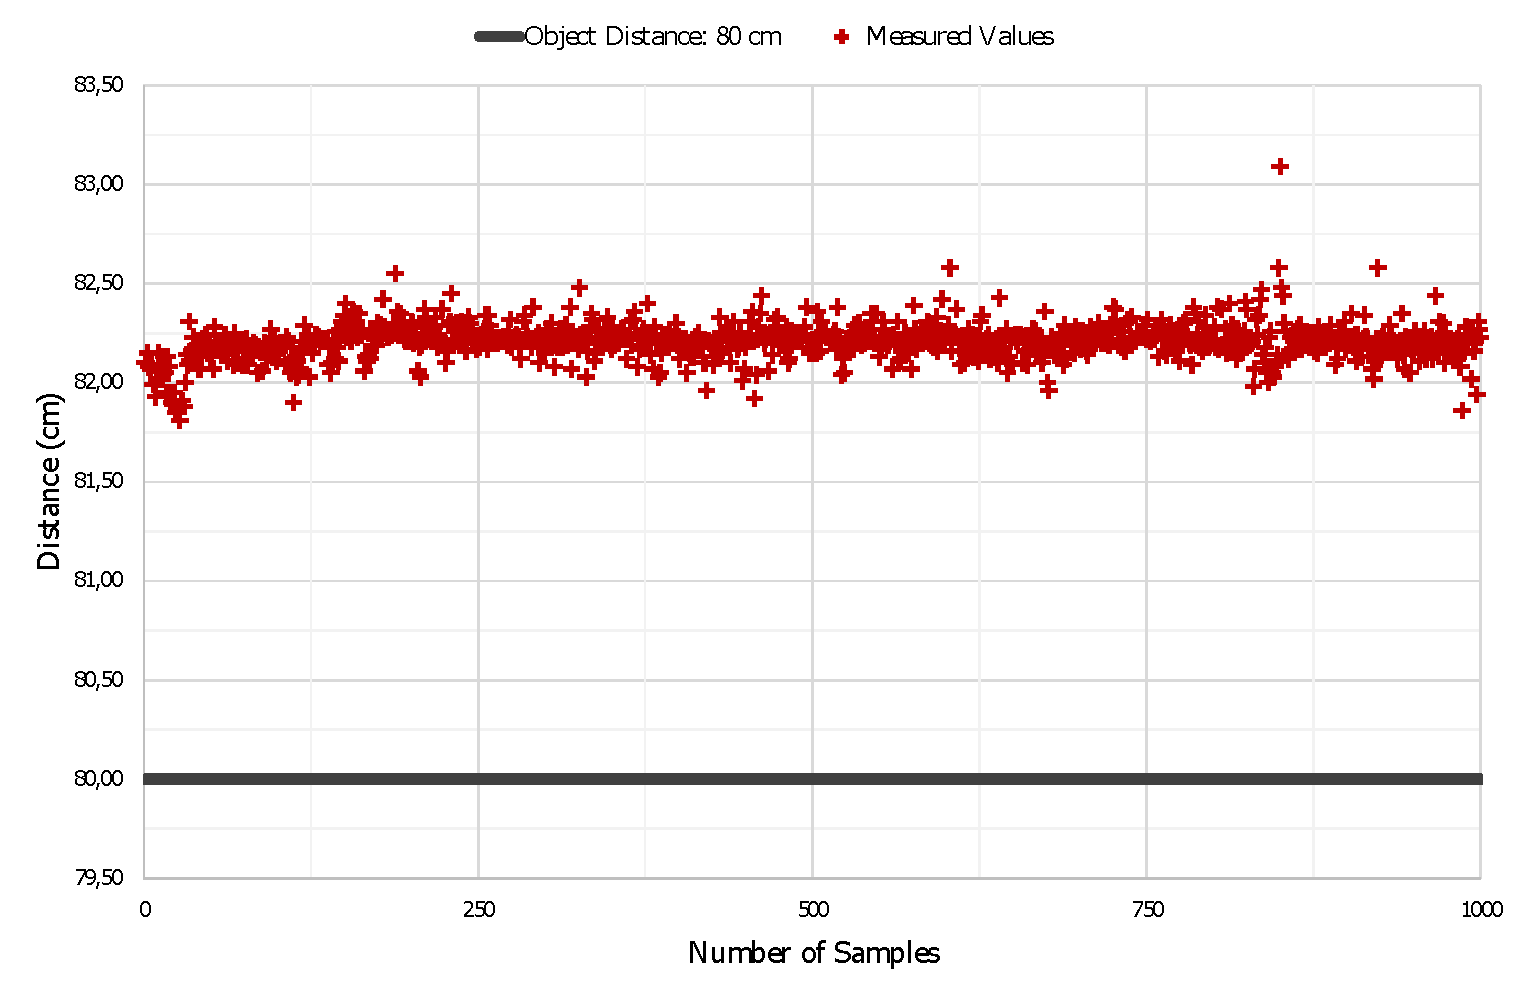
\includegraphics[scale=0.52]{images/Results/testing_methodology/conf80.pdf}
%     \caption{Analysis \#2; Object Distance: 80 cm.}
%     \label{fig:conf80}
% \end{figure}

% \begin{figure}[h!]
%     \centering
%     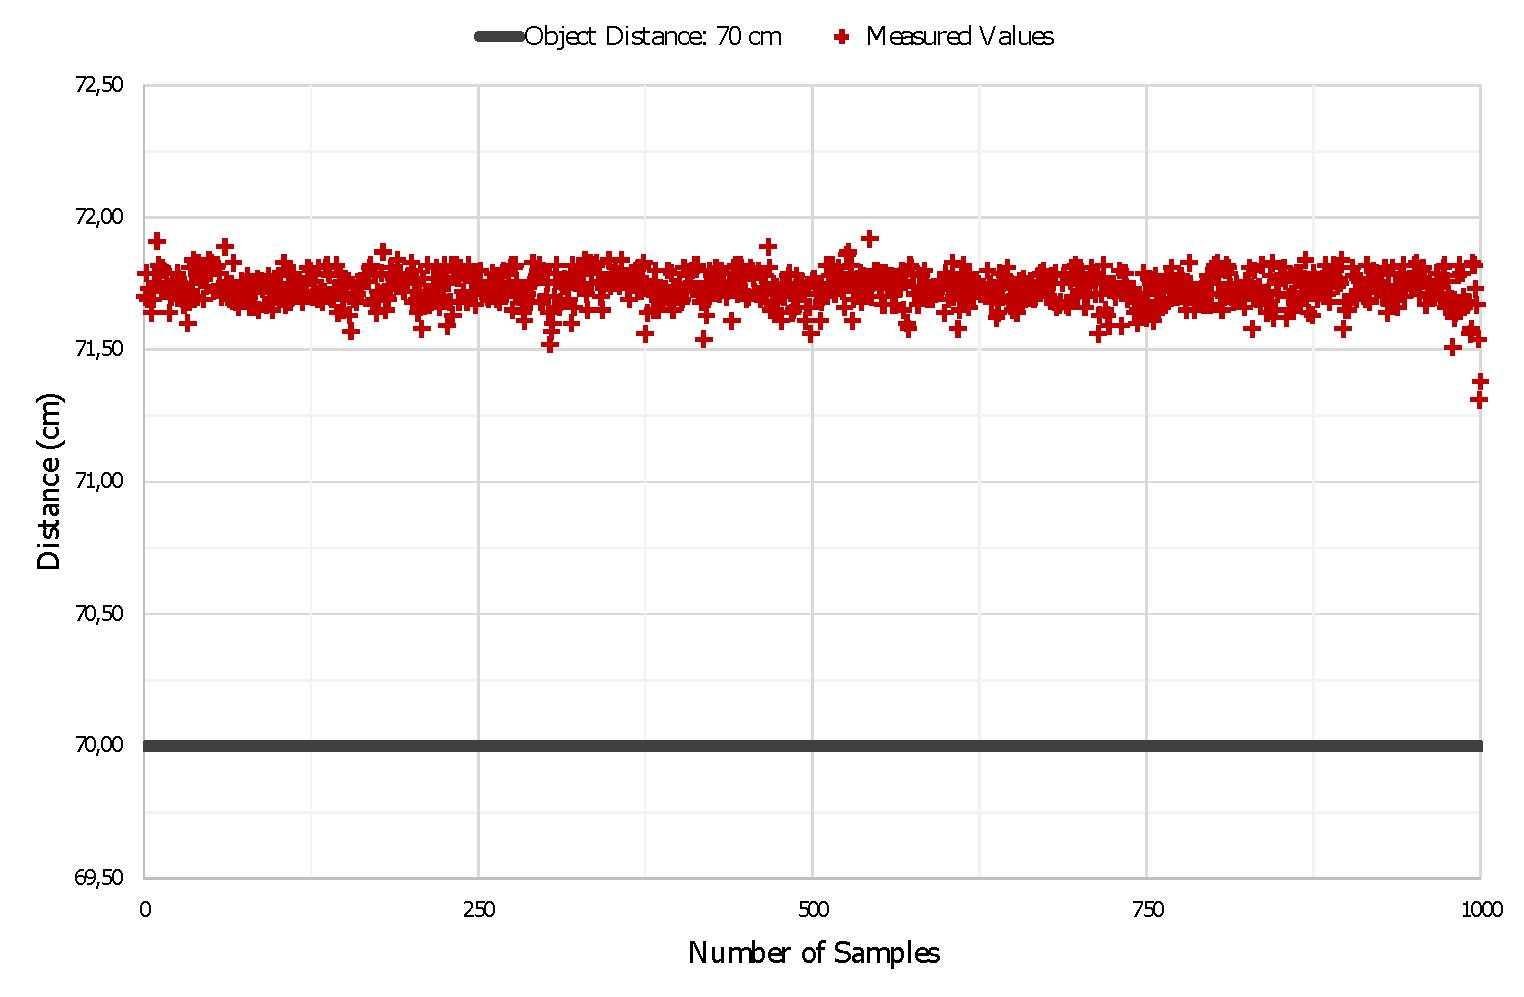
\includegraphics[scale=0.52]{images/Results/testing_methodology/conf70.pdf}
%     \caption{Analysis \#2; Object Distance: 70 cm.}
%     \label{fig:conf70}
% \end{figure}

% \begin{figure}[h!]
%     \centering
%     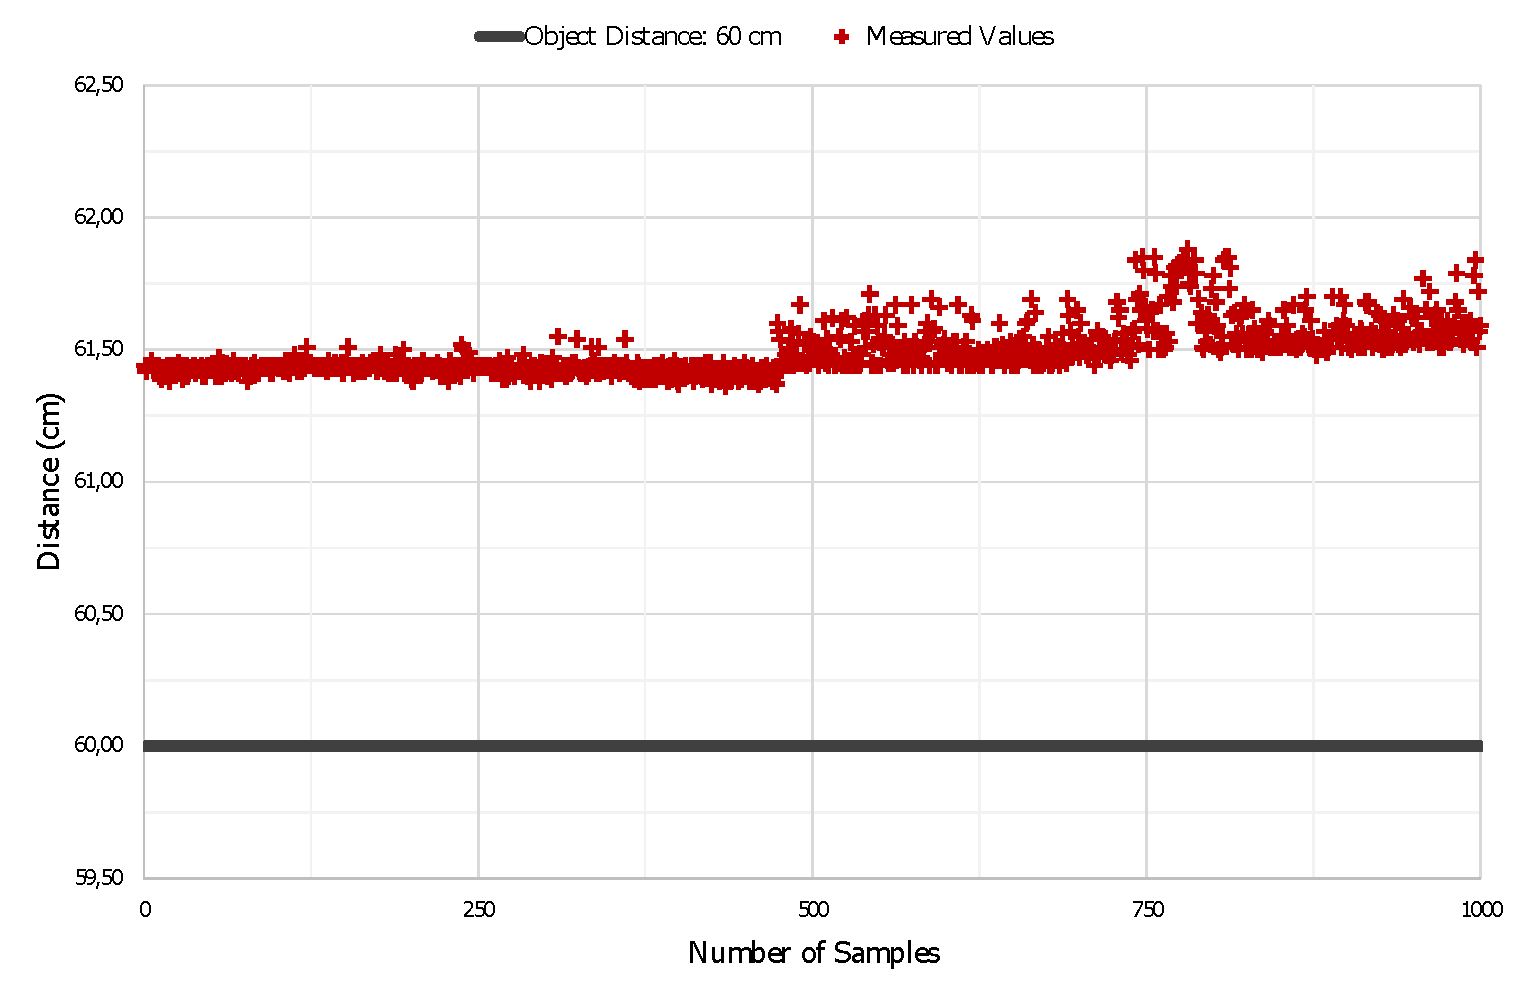
\includegraphics[scale=0.52]{images/Results/testing_methodology/conf60.pdf}
%     \caption{Analysis \#2; Object Distance: 60 cm.}
%     \label{fig:conf60}
% \end{figure}

% \begin{figure}[h!]
%     \centering
%     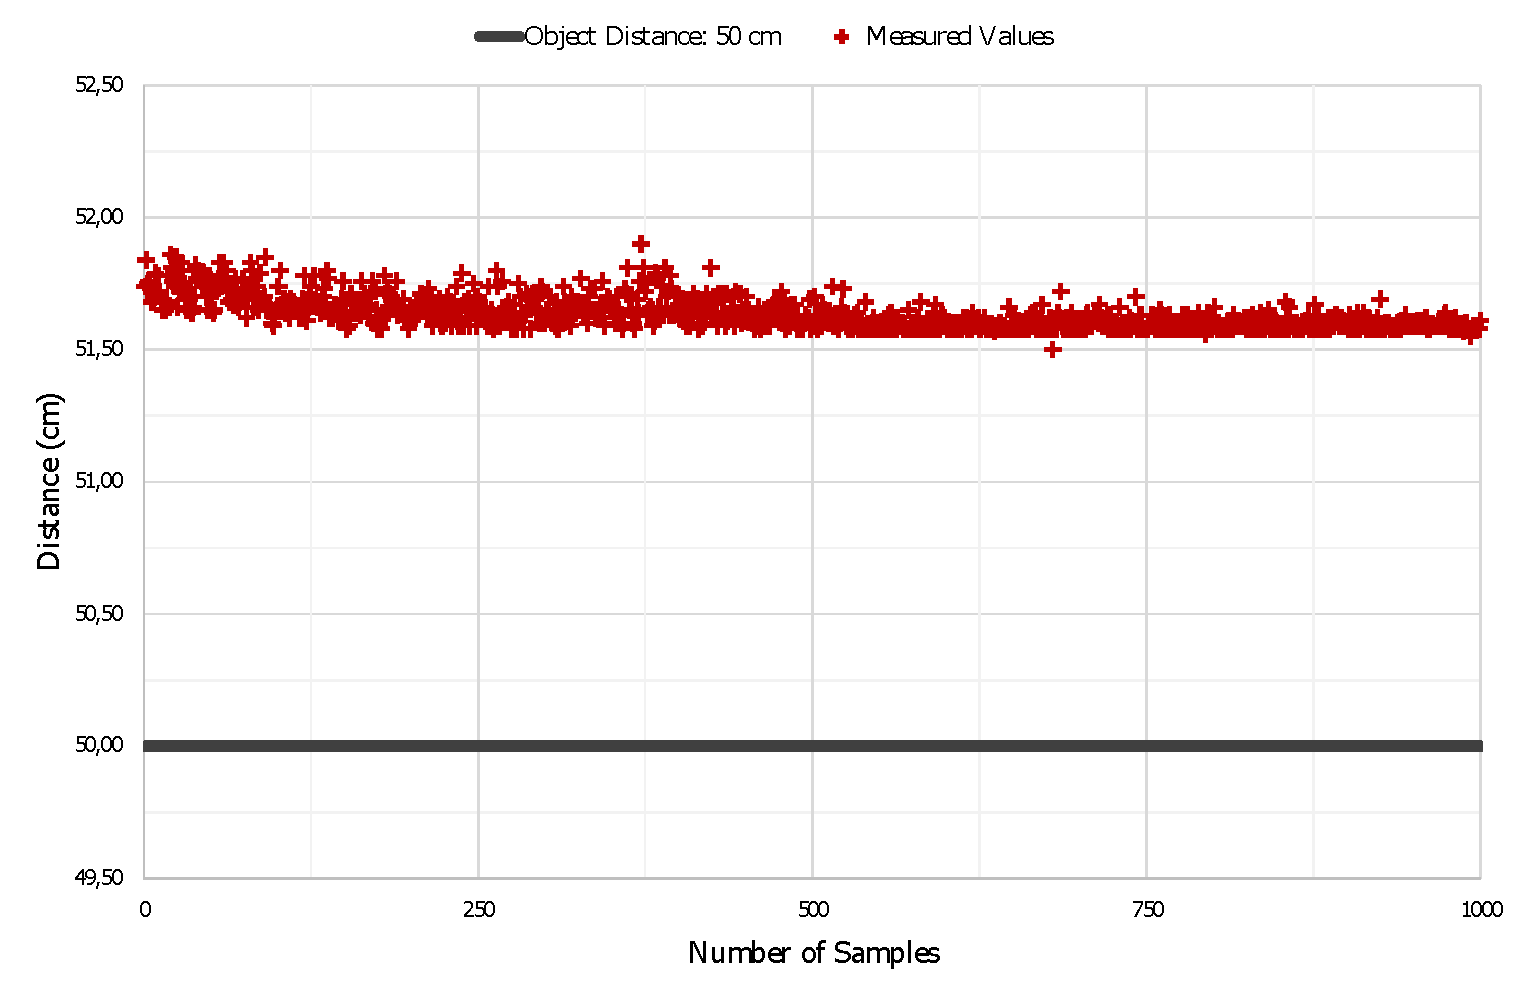
\includegraphics[scale=0.52]{images/Results/testing_methodology/conf50.pdf}
%     \caption{Analysis \#2; Object Distance: 50 cm.}
%     \label{fig:conf50}
% \end{figure}

% \begin{figure}[h!]
%     \centering
%     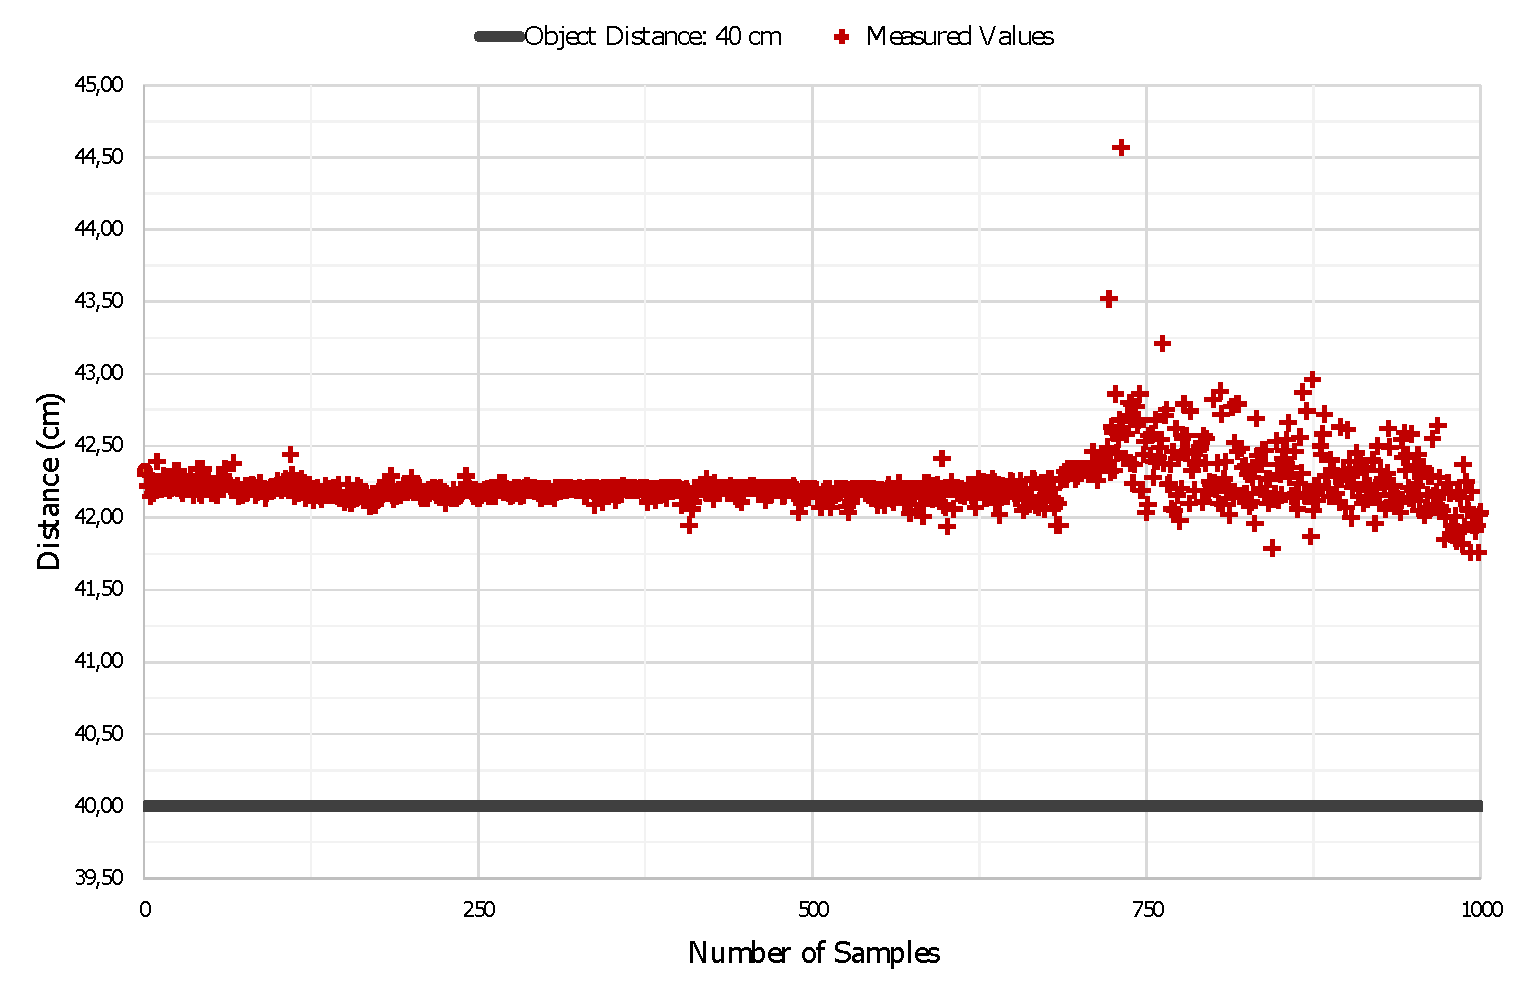
\includegraphics[scale=0.52]{images/Results/testing_methodology/conf40.pdf}
%     \caption{Analysis \#2; Object Distance: 40 cm.}
%     \label{fig:conf40}
% \end{figure}

% \begin{figure}[h!]
%     \centering
%     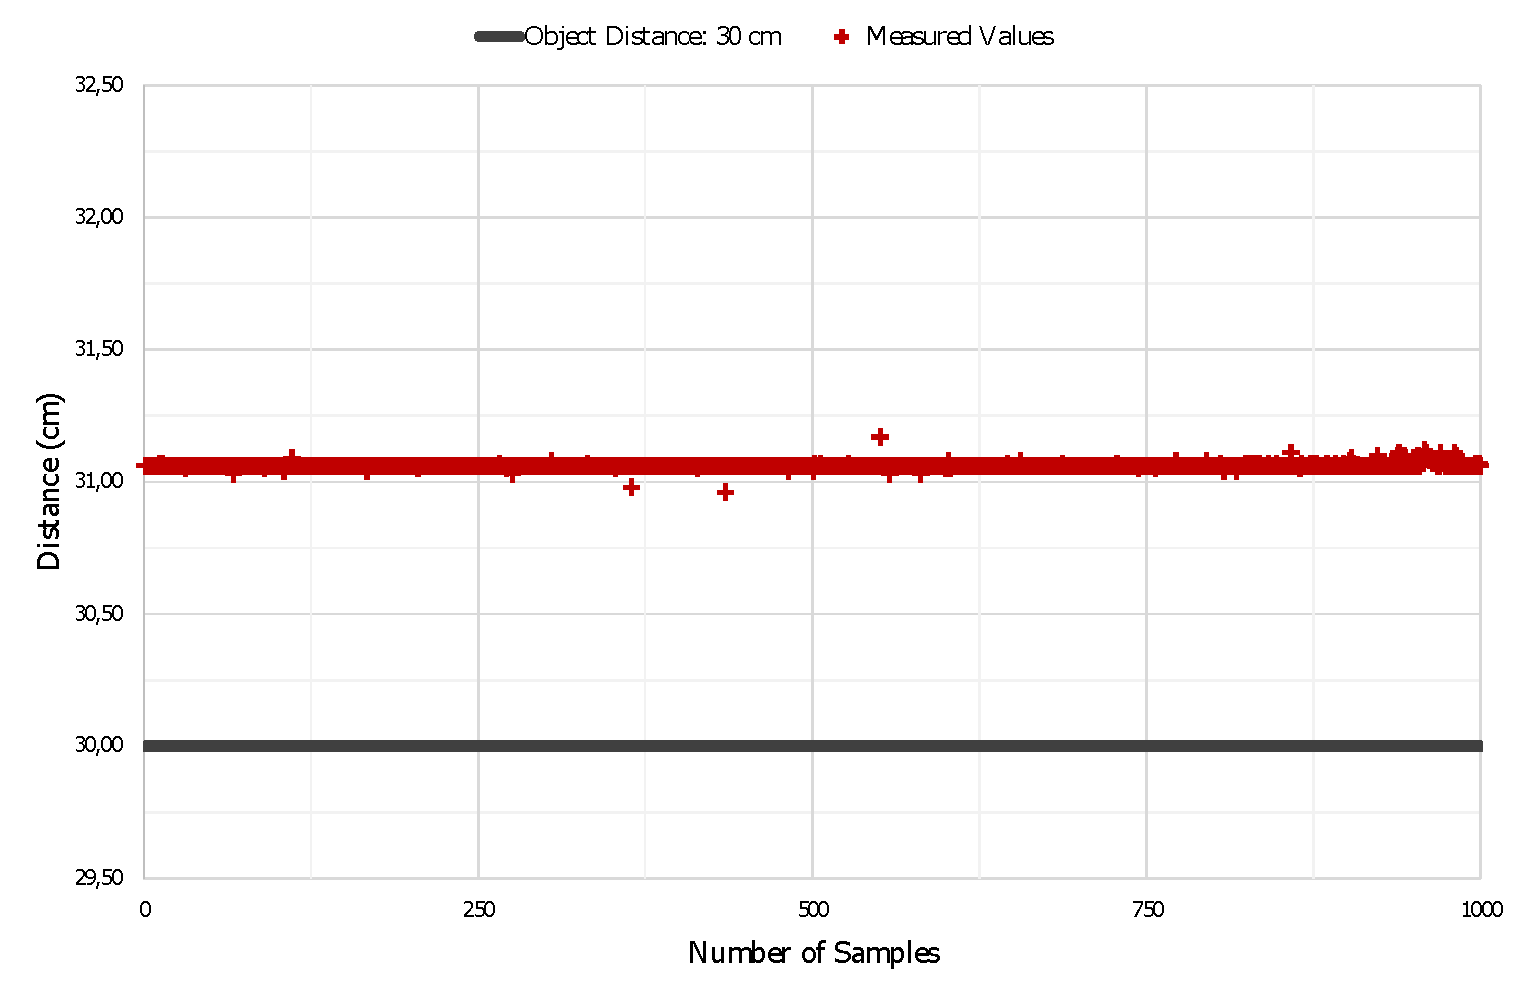
\includegraphics[scale=0.52]{images/Results/testing_methodology/conf30.pdf}
%     \caption{Analysis \#2; Object Distance: 30 cm.}
%     \label{fig:conf30}
% \end{figure}

% \begin{figure}[h!]
%     \centering
%     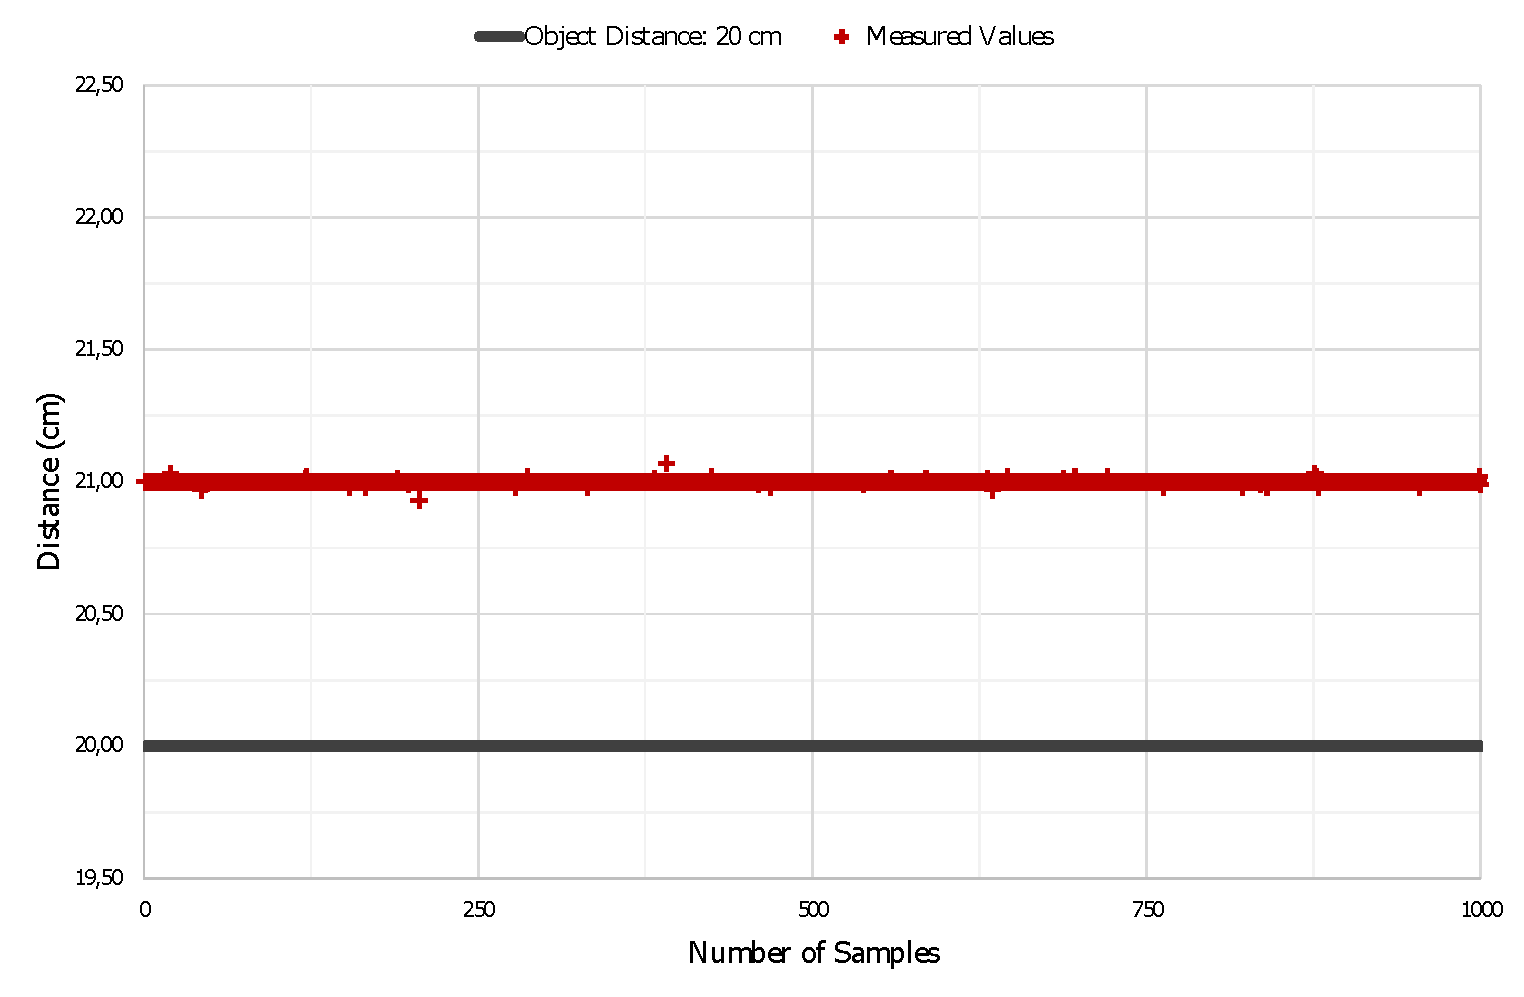
\includegraphics[scale=0.52]{images/Results/testing_methodology/conf20.pdf}
%     \caption{Analysis \#2; Object Distance: 20 cm.}
%     \label{fig:conf20}
% \end{figure}

% \begin{figure}[h!]
%     \centering
%     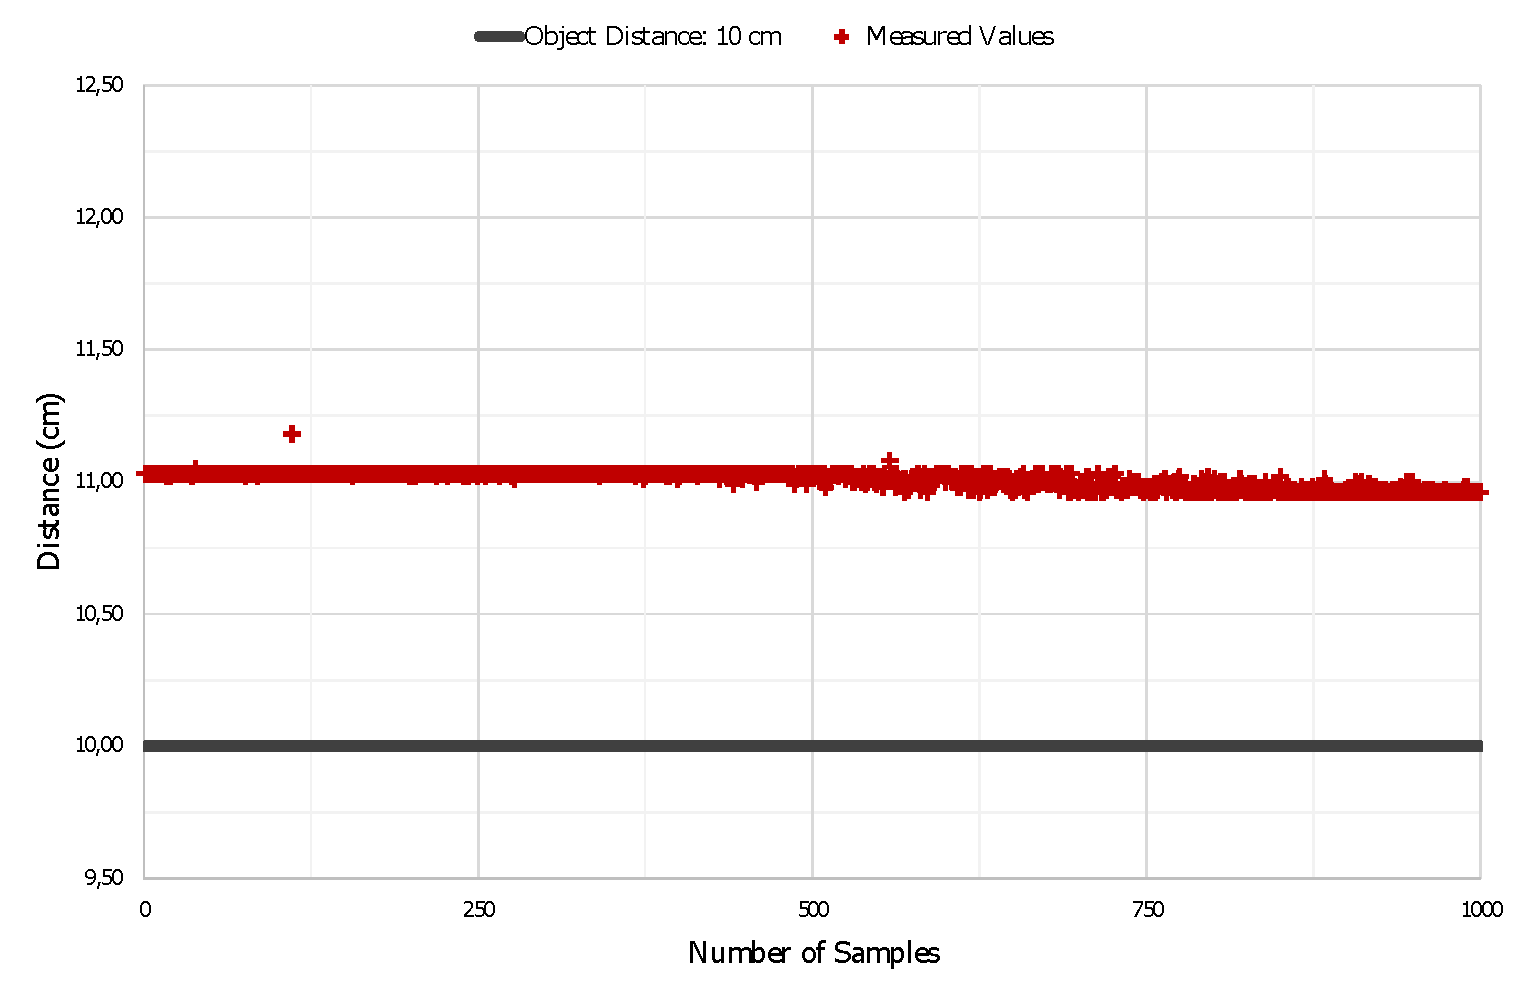
\includegraphics[scale=0.52]{images/Results/testing_methodology/conf10.pdf}
%     \caption{Analysis \#2; Object Distance: 10 cm.}
%     \label{fig:conf10}
% \end{figure}


% \clearpage
% \section{Temperature Influence}\label{appendice1:third}


% \begin{figure}[h!]
%     \centering
%     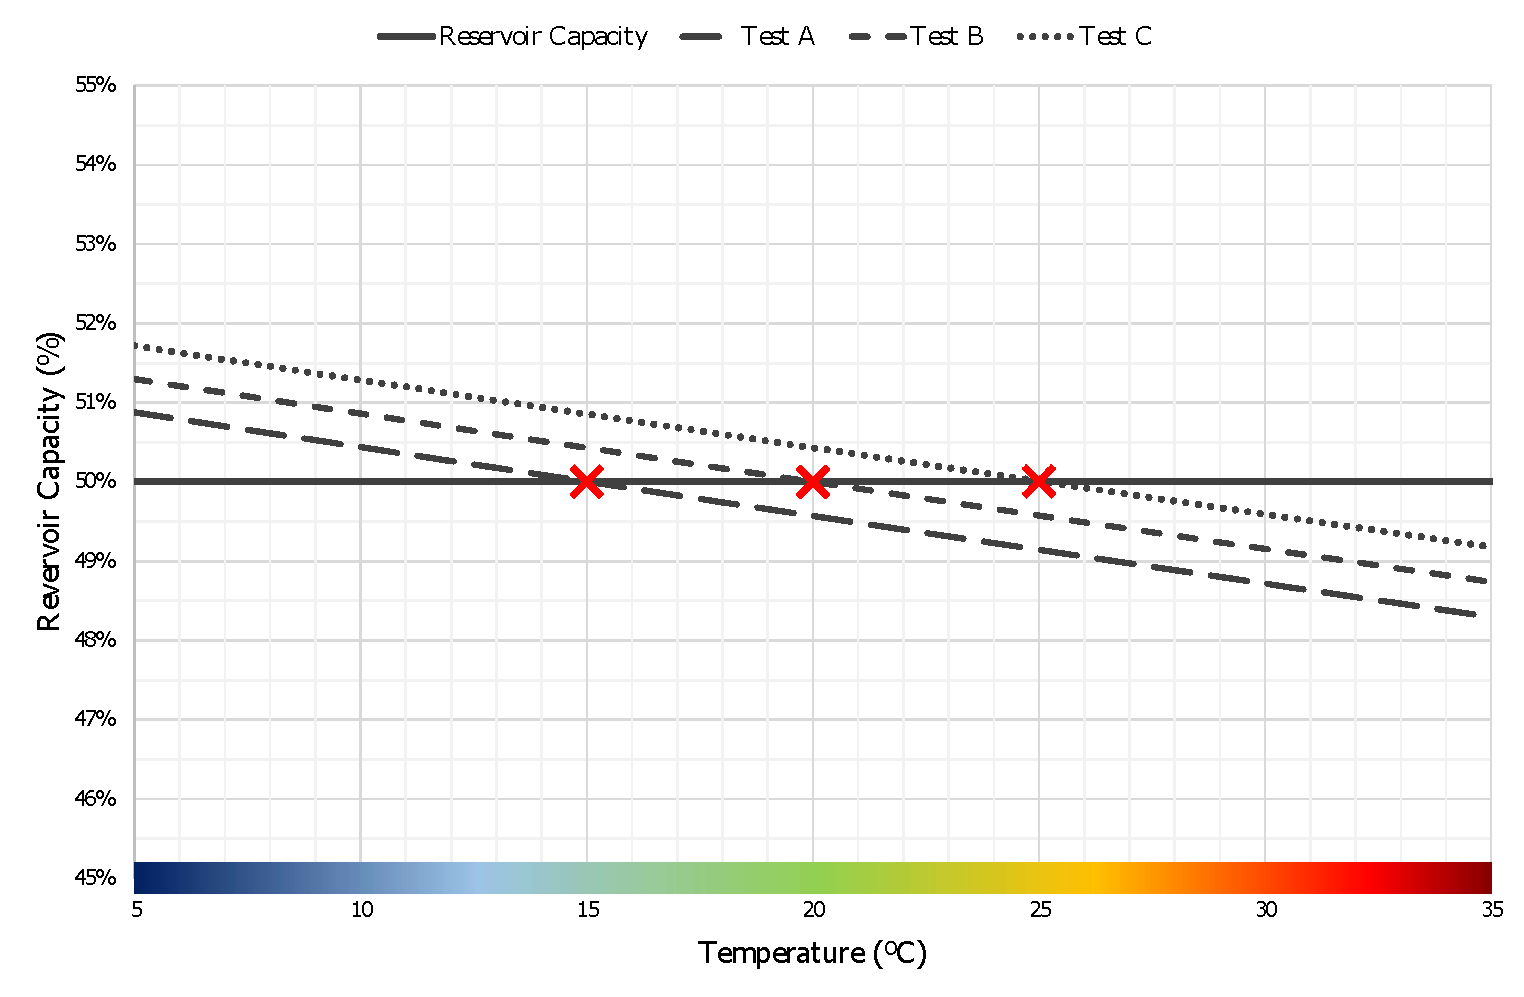
\includegraphics[scale=0.5]{images/Results/temperature_influence/Analyse_50.pdf}
%     \caption{Reservoir Capacity: 50 \%; Test A: 15ºC; Test B: 20ºC; Test C: 25ºC.}
%     \label{fig:ana50}
% \end{figure}

% \begin{figure}[h!]
%     \centering
%     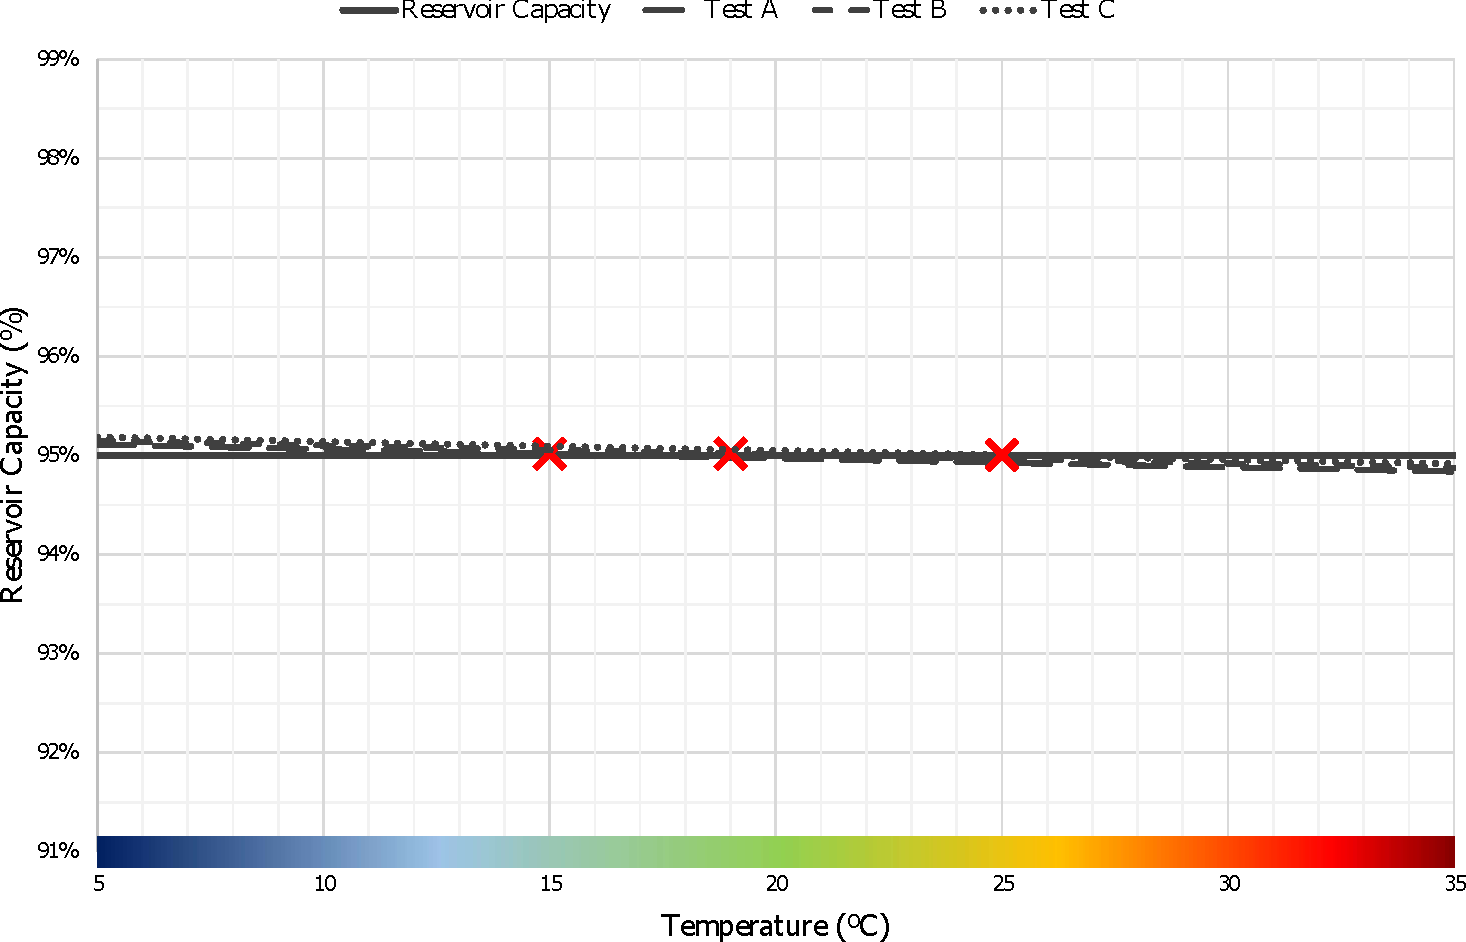
\includegraphics[scale=0.5]{images/Results/temperature_influence/Analyse_95.pdf}
%     \caption{Reservoir Capacity: 95 \%; Test A: 15ºC; Test B: 20ºC; Test C: 25ºC.}
%     \label{fig:ana95}
% \end{figure}


